%
%   Chapter Method
%
%   Qing-Cheng Li (r01922024 at csie dot ntu dot edu dot tw)
%   R.O.C.103.07
%
\chapter{研究方法}
\label{c:method}

本研究欲自內容串流中偵測實體的特性,
而實體的特性之一:實體間關係,則可以語句樣式表現,
因此本研究主要利用語句樣式來偵測這樣的特性是否存在。
本章節將介紹所使用的資源、
樣式比對、樣式篩選與特性歧異的問題與解決方法。

\section{以樣式偵測特性}
當我們在字裡行間要描述一個實體的特性時,
應該會有某些特定的樣式。
例如我們知道Jobs的出生地這個特性是San Francisco,
我們可能會以「Jobs was born in San Francisco」這樣的句子來表達這個概念。
而在上述句子之中「was born in」就是一個可以用來表示出生地此一實體特性的樣式,
當我們在句子中看到「was born in」時,就可以推測這個句子存在某人的出生地是某地這樣的實體特性。

基於這樣的想法,本研究將利用樣式的出現有無來決定是否存在實體特性,
設計了如圖\ref{i:process-v1}的偵測流程。

圖\ref{i:process-v1}中,首先要先有一份實體特徵與樣式的關聯表,
知道每個實體特徵可以由哪些樣式來表達。
再利用這份關係表,對文章中的句子進行比對,檢查關係表中的樣式是否有出現,
若有出現,則這篇文章可能包含樣式對映的實體特性。
樣式比對的細節會在第\ref{s:pattern-match}節中詳述。

\begin{figure}
    \centering
    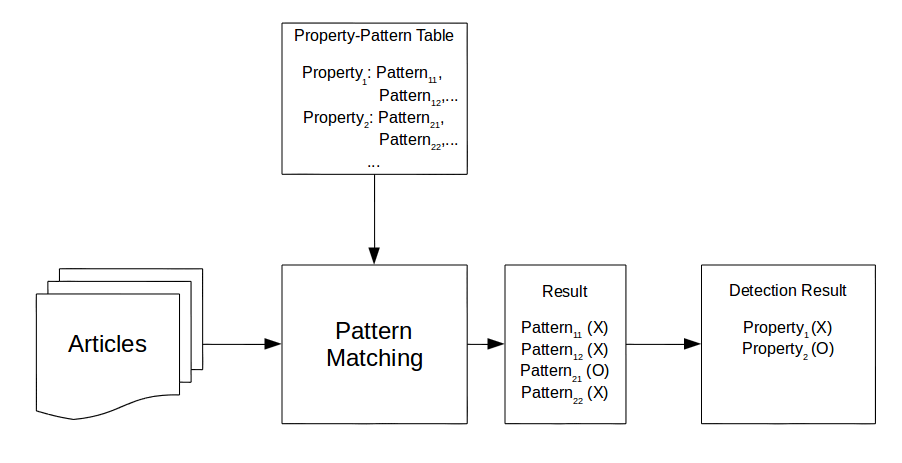
\includegraphics[width=0.9\textwidth]{images/03-process-v1}
    \caption{以樣式偵測特性流程概念}
    \label{i:process-v1}
\end{figure}

在這個流程之中,必須要有一份實體特徵與樣式的對映表。
此一部份本研究將利用PATTY已經提供的關係釋義表,
表中包含了知識庫YAGO內定義的實體間關係、
YAGO關係的領域與範圍(表\ref{t:yago-relation}),
以及可以用來描述這個關係的樣式。

%t:yago-relation
\begin{table}[t]
    \begin{center}
        \footnotesize
        \begin{tabular}{|l||c|c|c|}
        \hline
        YAGO Relation & Domain & Range & Number of patterns \\
        \hline
        actedIn & wordnet\_actor & wordnet\_movie & 2023 \\
        created & yagoLegalActor & Thing & 3215 \\
        dealsWith & wordnet\_location & wordnet\_location & 366 \\
        diedIn & wordnet\_person & wordnet\_city & 1352 \\
        directed & wordnet\_person & wordnet\_movie & 1228 \\
        graduatedFrom & wordnet\_person & wordnet\_university & 2129 \\
        happenedIn & wordnet\_event & yagoGeoEntity & 47 \\
        hasAcademicAdvisor & wordnet\_person & wordnet\_person & 632 \\
        hasCapital & wordnet\_location & wordnet\_location & 24 \\
        hasChild & wordnet\_person & wordnet\_person & 3620 \\
        hasWonPrize & yagoLegalActorGeo & wordnet\_award & 78 \\
        holdsPoliticalPosition & wordnet\_person & wordnet\_person & 1173 \\
        influences & wordnet\_person & wordnet\_person & 2461 \\
        isCitizenOf & wordnet\_person & wordnet\_country & 813 \\
        isKnownFor & yagoLegalActor & Thing & 1574 \\
        isLeaderOf & wordnet\_person & yagoLegalActorGeo & 465 \\
        isLocatedIn & yagoPermanentlyLocatedEntity & yagoGeoEntity & 1300 \\
        isMarriedTo & wordnet\_person & wordnet\_person & 4276 \\
        isPoliticianOf & wordnet\_person & wiki\_states\_of\_US & 465 \\
        livesIn & wordnet\_person & wordnet\_location & 718 \\
        participatedIn & yagoLegalActorGeo & Thing & 89 \\
        playsFor & wordnet\_person & wordnet\_organization & 1491 \\
        wasBornIn & wordnet\_person & wordnet\_city & 1226 \\
        worksAt & wordnet\_person & wordnet\_organization & 1602 \\
        \hline
        \end{tabular}
        \caption{YAGO Relations in PATTY}
        \label{t:yago-relation}
    \end{center}
\end{table}


光是這樣的流程並不足以偵測實體特性。
使用樣式來偵測實體特性還會有樣式覆蓋度(Coverage)、
品質(Quality)、可信賴度(Reliability)與歧異性(Ambiguity)的問題。

樣式覆蓋度問題是指對於某個實體的特性,
在關係表內屬於這個實體特性的樣式佔所有可以表達該特性的樣式之比例。
例如一個實體特性可以用100種樣式來描述,
但只找出了其中70種,
這樣就沒有辦法找到以其他30種樣式來描述該特性的句子。

樣式的品質則是一個字串到底能不能夠作為一個樣式,    %FIXME
一個樣式的品質不高,那麼這樣的樣式有可能太廣泛的出現在句子之中,
致使這樣的樣式沒有辦法區辨出實體屬性。
例如PATTY關係釋義中的DBpedia:manager內的樣式「hired」就只有這一個單字,
用以描述實體特性顯得太廣泛了些,
以此擷取回的文章有包含實體特性的比例就較低。

樣式可信賴度則是一個樣式到底能不能用來表達實體特性。
例如,對於特性YAGO:diedIn,以「since worked in」來描述完全文不對題。

而為了處理樣式的品質、可信賴度問題,
應該要在圖\ref{i:process-v1}流程中的關聯表與樣式比對中增加一個樣式篩選的步驟,
篩選出可信賴、有一定品質的樣式來進行樣式比對,
此部份將於第\ref{s:select-pattern}小節說明詳細內容。

經過樣式比對後,每篇文章可能存在數個樣式,
如果在關聯表中每個樣式只對映到一個關係,
那便沒有歧義。
但一個樣式可能存在於多個實體特性的關聯表內,
例如樣式「first met with」就被PATTY認為可以表示5種特性(hasAcademicAdvisor、isKnownFor、isMarriedTo、influences、hasChild)。
因此在樣式被比對出來之後,整個偵測流程中還需要一個消歧義的步驟。
這個部份將在第\ref{s:pattern-disambiguity}節中說明。

補上了樣式篩選與消歧義後的流程圖應修正為圖\ref{i:process-v2}。
樣式比對使用的樣式是經過篩選的,
比對出來後還要進行消歧義才完成偵測實體特性之流程。
由於偵測實體特性的流程對於每一分文件都是相同,且彼此互相獨立,
因此可以平行處理文件,如圖\ref{i:process-parallel}所示,
處理內容串流的大量文件。

\begin{figure}
    \centering
    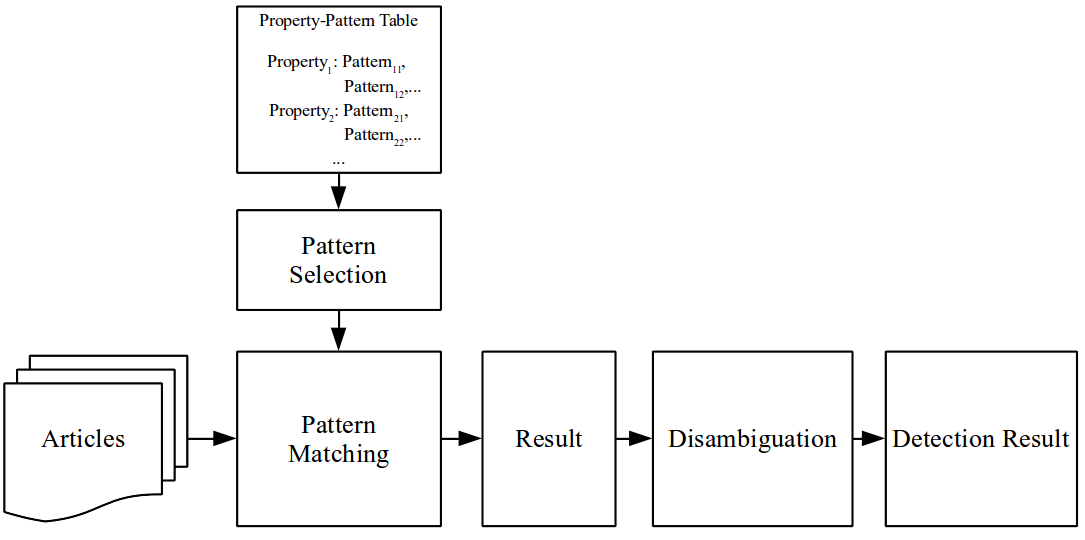
\includegraphics[width=0.9\textwidth]{images/03-process-v2}
    \caption{以樣式偵測特性流程}
    \label{i:process-v2}
\end{figure}

\begin{figure}
    \centering
    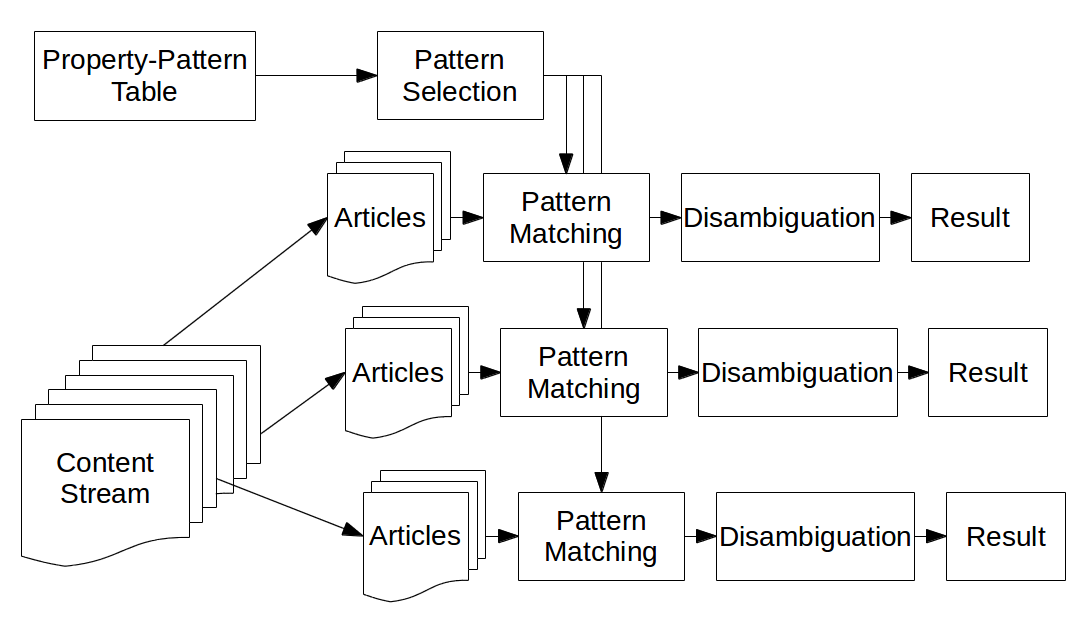
\includegraphics[width=1\textwidth]{images/03-pattern-parallel}
    \caption{平行處理架構}
    \label{i:process-parallel}
\end{figure}

\section{樣式比對}
\label{s:pattern-match}

樣式比對是要從句子之中確定某一個樣式是否存在,
PATTY中提供的25個YAGO關係有43,124個樣式,
但其中有不少是重複出現的,
實際上總共有19,031個獨特的樣式,
如果對每個句子都做19,031次比較顯然不是一個好方法。

% Prefix-Tree
為了讓樣式比對可以有效率些,
我們將所有的樣式建立成一顆前綴樹(Prefix Tree)。
先將所有首字相同的樣式合併成同一個節點,
再看第二個字是否相同,如果不同就分支出去,
以此類推,最後再連結到樣式編號,
即可透過編號查詢該樣式可能表示的實體特性。
如圖\ref{i:pattern-prefix-tree}所示,
四個樣式「was born」、「was born at」、「was born [[det]] village」和「was bron [[det]] willage in」的首字皆為was,所以併成一個節點。
第二個字也都相同,所以也併成一個節點。
而此時「was born」已經完成了,所以born節點下新增一個樣式編號的節點。
剩下三個樣式的第三個字有詞性標記「[[det]]」和單字「at」,
便在born節點下新增[[det]]和at節點。at節點完成了「was bron at」樣式,
而[[det]]節點則繼續將後續的字加入這棵前綴樹上,
最後這棵樹上所有葉子都是一個樣式編號。

\begin{figure}
    \centering
    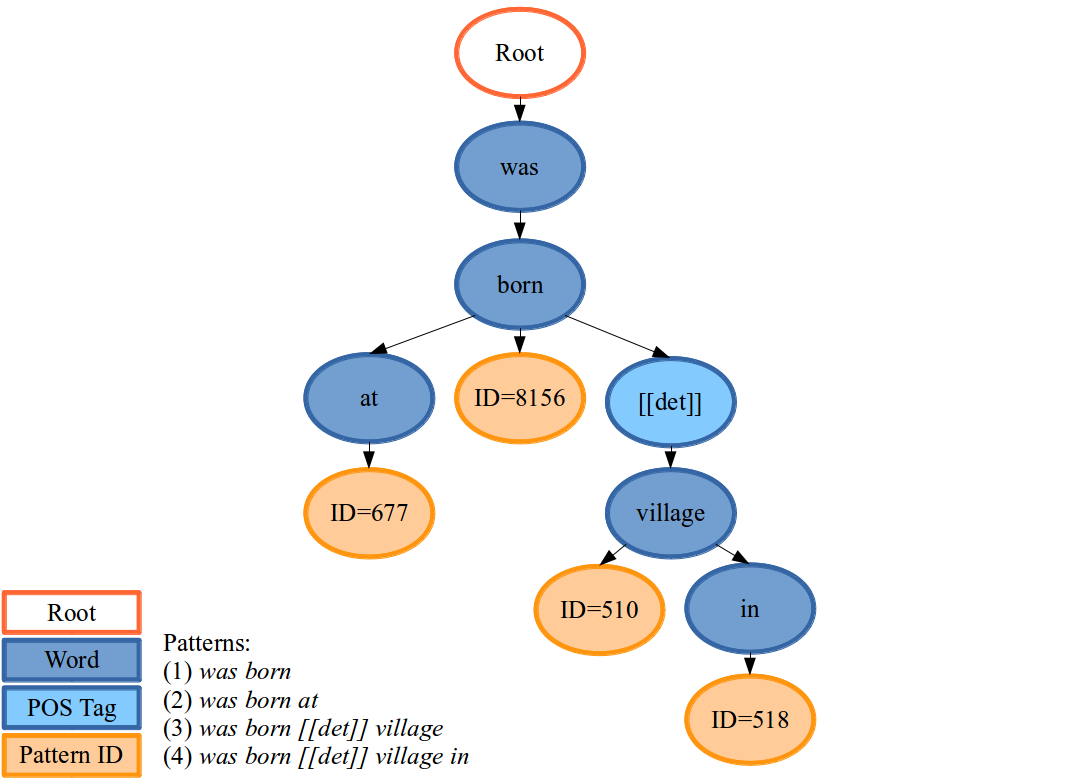
\includegraphics[width=0.9\textwidth]{images/03-pattern-prefix-tree}
    \caption{樣式前綴樹}
    \label{i:pattern-prefix-tree}
\end{figure}

% Algo
有了樣式前綴樹後,
再來就是利用這棵樹來比對句子中是否有出現其中的樣式。
演算法\ref{a:pattern-match}描述了比對的過程。

演算法\ref{a:pattern-match}的輸入是欲比對的文章A以及已經預先建立完成的樣式前綴樹T,
輸出是文章A所出現過的樣式及其出現的位置。
對於文章A中的每個句子S,由於樣式包含詞性標記,
因此需要將S標記,實驗中使用的是Textblob的APTagger\footnote{https://github.com/sloria/textblob-aptagger}來進行快速的詞性標記。
接下來開始從句子的第一個字開始,
如果這個字或其詞性標記有出現在樣式前綴樹Root下的第一層節點中出現,
便將這個節點和此字於句子中的位置記錄下來。
再看句子中的下一個字,
此時先檢查暫存紀錄中的字是不是能夠繼續往下走這棵樣式前綴樹,
如果可以往下走代表還沒有發現樣式;
如果子節點已經是帶有樣式編號的樹葉的話,
就是發現了一個樣式,然後紀錄下來。
如果發現沒有辦法繼續往下走,
則代表在未來的步驟中不可能走到任何一個紀錄樣式編號的樹葉,
因此將這組紀錄從暫存紀錄中移除。
最後便可以知道有哪些樣式出現在文章中以及出現的位置。

\begin{algorithm}
    \caption{樣式比對演算法}
    \label{a:pattern-match}
    \begin{algorithmic}[1]
        \Require  
            $A$: 文章;
            $T$: 樣式前綴樹;
        \Ensure
            $P$: 文章$A$中出現的樣式;
        \State $P\gets$[]
        \Comment{初始化$P$}
        \ForAll{Sentence $S$ {\bf in} $A$ }
            \State 對$S$進行詞性標記
            \State $tmpP\gets$[]
            \Comment{初始化暫存陣列}
            \For{$i$ {\bf from} 0 to length of $S$}
                \State ($word$,$POStag$) $\gets$ $S[i]$
                \ForAll{$possiblePattern$ {\bf in} $tmpP$}
                    \If{$word$ or $POStag$ {\bf in} $T$'s $possiblePattern$.depthInTree+1 level nodes}
                        \State continue
                    \Else
                        \If{$T$'s $possiblePattern$.depthInTree+1 level node is $PatternID$}
                            \State {\bf add} ($PatternID$,$startPoint$,$i$ as $endPoint$) {\bf into} $P$
                        \EndIf
                        \State {\bf remove} $possiblePattern$ {\bf from} $tmpP$
                    \EndIf
                \EndFor
                \If{$word$ or $POStag$ {\bf in} $T$'s first level nodes}
                \State {\bf add} ($depthInTree$,$i$ as $startPoint$) {\bf into} $tmpP$
                \EndIf
            \EndFor
        \EndFor
        \State \Return P
    \end{algorithmic}
\end{algorithm}

演算法\ref{a:pattern-match}中同時於暫存紀錄中的可能樣式最多只會跟樣式前綴樹的深度相同,若文章的長度是n個字、前綴樹深度m,則演算法\ref{a:pattern-match}的時間複雜度是O(mn)。

\section{樣式篩選}
\label{s:select-pattern}

\section{特性消歧義}
\label{s:pattern-disambiguity}

% Pattern Extraction
% Pattern Matching
%   O(mn)?
% Some statistics e.g. how many pattern, how long, ...etc

